\section{Data}

The data was being gathered using the IDE plugin called \texttt{MIMUW-MB-TT} \ref{sec:context} in the period between 10th October and 25th November 2022. 15 programmers participated in the research. They usually contributed information about at least a few of their working days \ref{fig:data_by_date}. Majority of the data related to Python and JavaScript/TypeScript (JS/TS) languages \ref{fig:data_by_langs}. JavaScript (JS) and TypeScript (TS) are treated as one language later in my analysis due to their similarity (TS is a typed superset of JS) and the fact that TS is transpiled to (plain) JS \cite{Mic22CompilingTS}.

\begin{figure}[htbp]
  \centering
  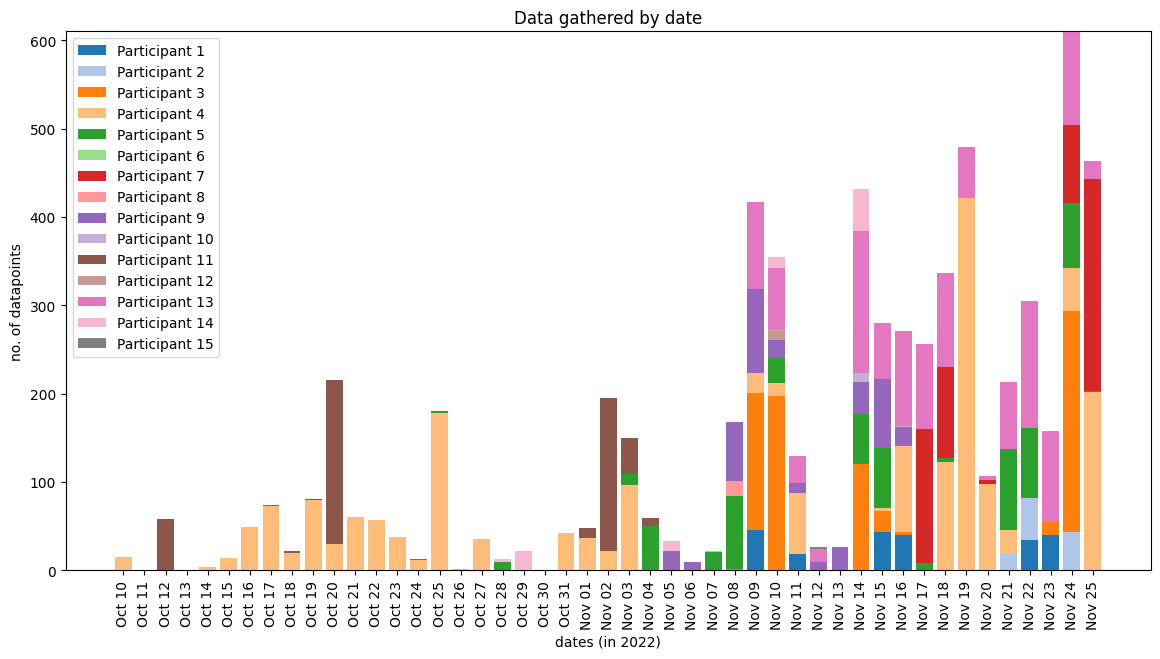
\includegraphics[scale=0.5]{chapters/methodology/graphics/data-gathered-dates.png}
  \caption{Data gathered from participants by date}
  \label{fig:data_by_date}
\end{figure}

\begin{figure}[htbp]
  \centering
  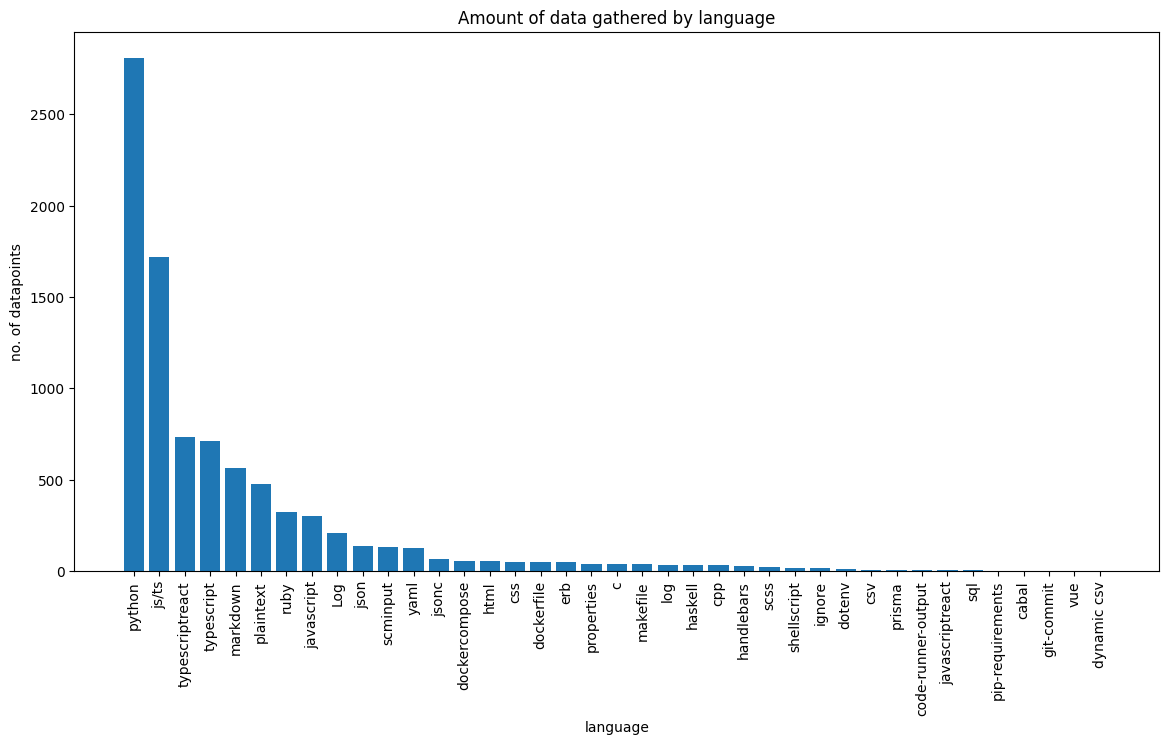
\includegraphics[scale=0.5]{chapters/results/graphics/languages-total.png}
  \caption{Amount of data gathered by language}
  \label{fig:data_by_langs}
\end{figure}
